\documentclass[presentation]{beamer}   % to compile the presentation
% \documentclass[handout]{beamer}        % to compile 2x2 handouts
\usepackage[ansinew]{inputenc}
\usepackage[T1]{fontenc}
\usepackage{lmodern,textcomp}
\usepackage{breakurl}

\usetheme{dtu}

\graphicspath{{../img/diagrams/}}

\newcommand{\comm}[1]{}
\AtBeginSection[]
{
 \begin{frame}<beamer>
 \frametitle{Outline}
 \tableofcontents[currentsection]
 \end{frame}
}


\newcommand {\framedgraphic}[2] {%
    \begin{frame}{#1}%
        \begin{center}%
            \includegraphics[width=1.0\textwidth,height=0.75\textheight,keepaspectratio]{#2}%
        \end{center}
    \end{frame}
}

\begin{document}

% The DTU and MIC logos
\pgfdeclareimage[height=2cm]{dtulogo}{dtu_logo}
\pgfdeclareimage[width=0.8\framesep]{miclogo}{mic_logo}

\author{Mikkel \textsc{Bojsen}, Johan van \textsc{Beusekom}, Andreas \textsc{Foldager}, Kasper \textsc{Johansen}, Martin \textsc{Tange}}
\title{System Integration Project Presentation}
\date{May 31st}
\institute[%
  Compute
  ]{%
  DTU -- Technical University of Denmark
}
% \titlegraphic{\pgfuseimage{dtulogo}} % Graphics for title slide
%\logo{\pgfuseimage{miclogo}} % The left logo

\begin{frame}
  \maketitle
\end{frame}

% % % % % % % % % % % % % % % % % % % % % % % % % % % % % % % % % % % % % % % % % % % % % % % % % %

\section{Introduction}

\begin{frame}{Business processes}
Toll tag example:
\begin{figure}[H]
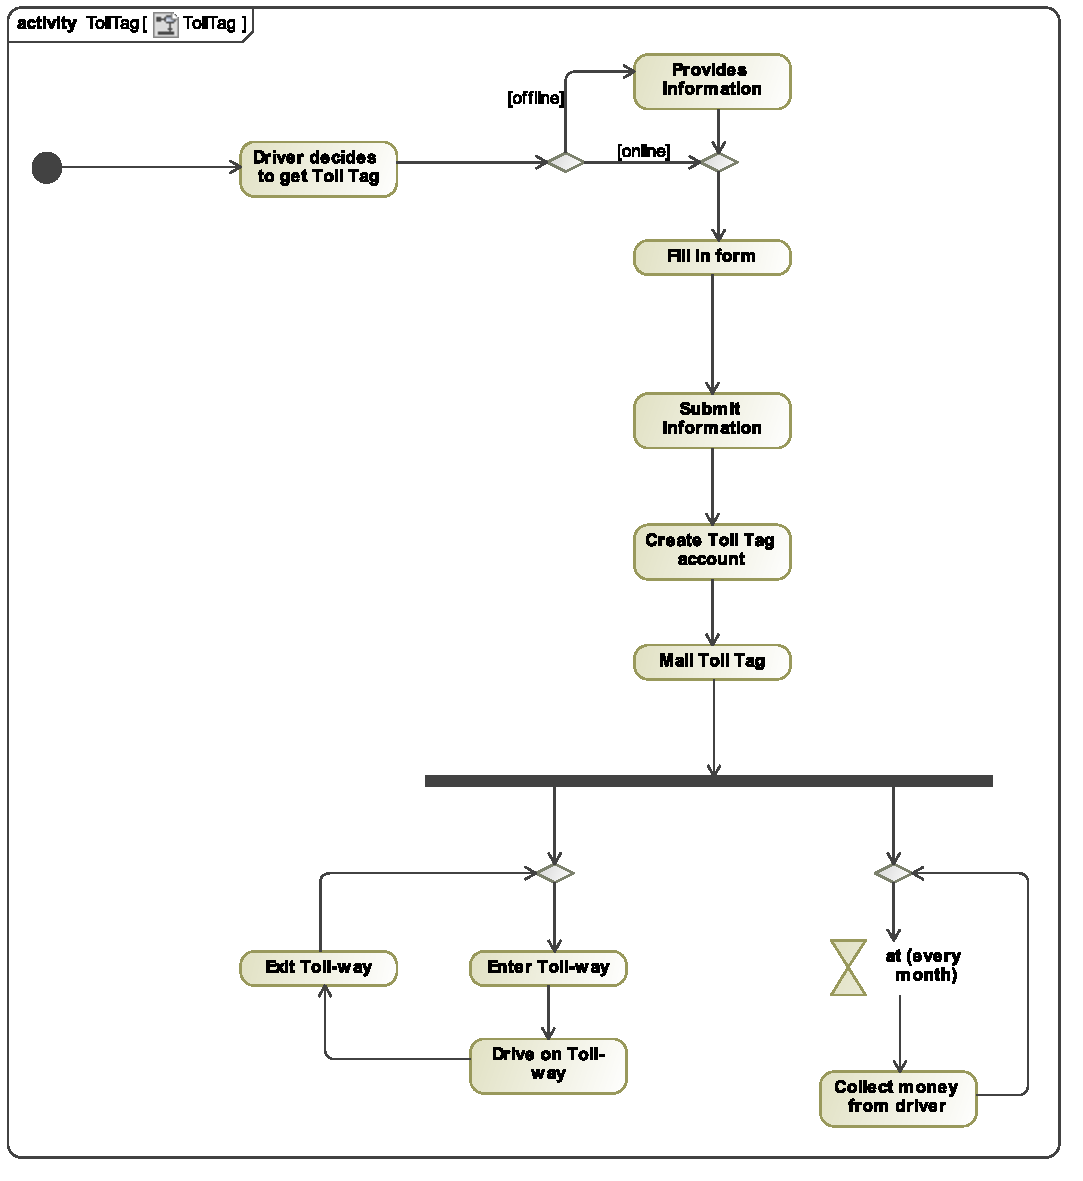
\includegraphics[width=\textwidth,height=0.7\textheight,keepaspectratio]{Activity_Diagram/TollTag}
\end{figure}
\end{frame}

\begin{frame}{Priority of use cases}
\begin{itemize}
\item Ticket check-in
\item Ticket check-out
\item Toll tag check-in
\item Toll tag check-out
\item Generate reports
\end{itemize}
\end{frame}

\begin{frame}{Use cases}
toll tag - check-in/check-out %TODO KASPER SKRIVER
\begin{figure}[H]
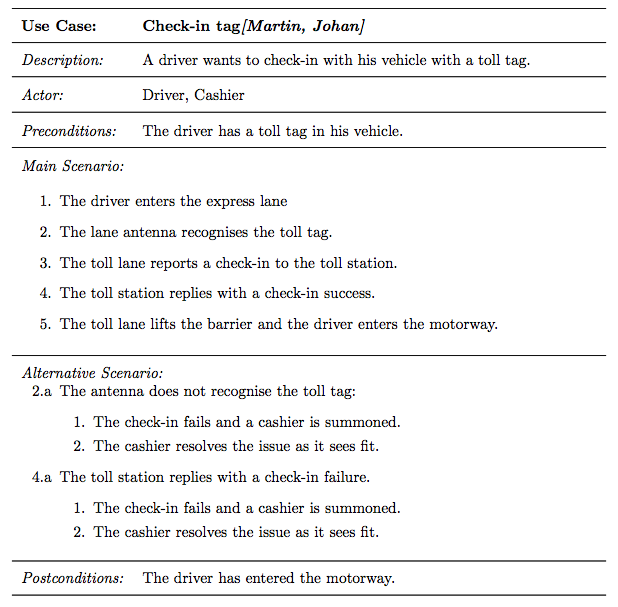
\includegraphics[width=\textwidth,height=0.7\textheight,keepaspectratio]{checkInTag}
\end{figure}
\end{frame}


\framedgraphic{Domain model}{Class_Diagram/Domain_Diagram}


% % % % % % % % % % % % % % % % % % % % % % % % % % % % % % % % % % % % % % % %

\section{Overall Design}

\begin{frame}{Assumptions}
\begin{itemize}
\item Barrier functionality
\item Bank communication
\item Security
\item Buy Toll tag implementation
\end{itemize}
\end{frame}

\framedgraphic{Component Interfaces}{Implementation_Diagram/Component_with_Interfaces}
\framedgraphic{TollLane Interfaces}{Implementation_Diagram/TollLane_with_Interfaces}


% % % % % % % % % % % % % % % % % % % % % % % % % % % % % % % % % % % % % % % % % % % % % %

\section{Detailed Design}


\framedgraphic{Class Diagram Overall}{Class_Diagram/Class_Diagram}

\framedgraphic{Class Diagram Lane \& Peripherals}{Class_Diagram/Lane+Peripherals}

\framedgraphic{OCL: Check-in lane}{Class_Diagram/OCLCheckInLane}

\framedgraphic{OCL: Enterprise Report}{Class_Diagram/OCLEnterpriseReport}



% % % % % % % % % % % % % % % % % % % % % % % % % % % % % % % % % % % % % % % % % % % % % %

\section{Behavior Design}


\framedgraphic{State Machine: Check-in Lane}{State_Machine_Diagram/CheckInLane}


\begin{frame}{State Machine: Check-in Lane}%
\vspace{-8mm}
\begin{center}%
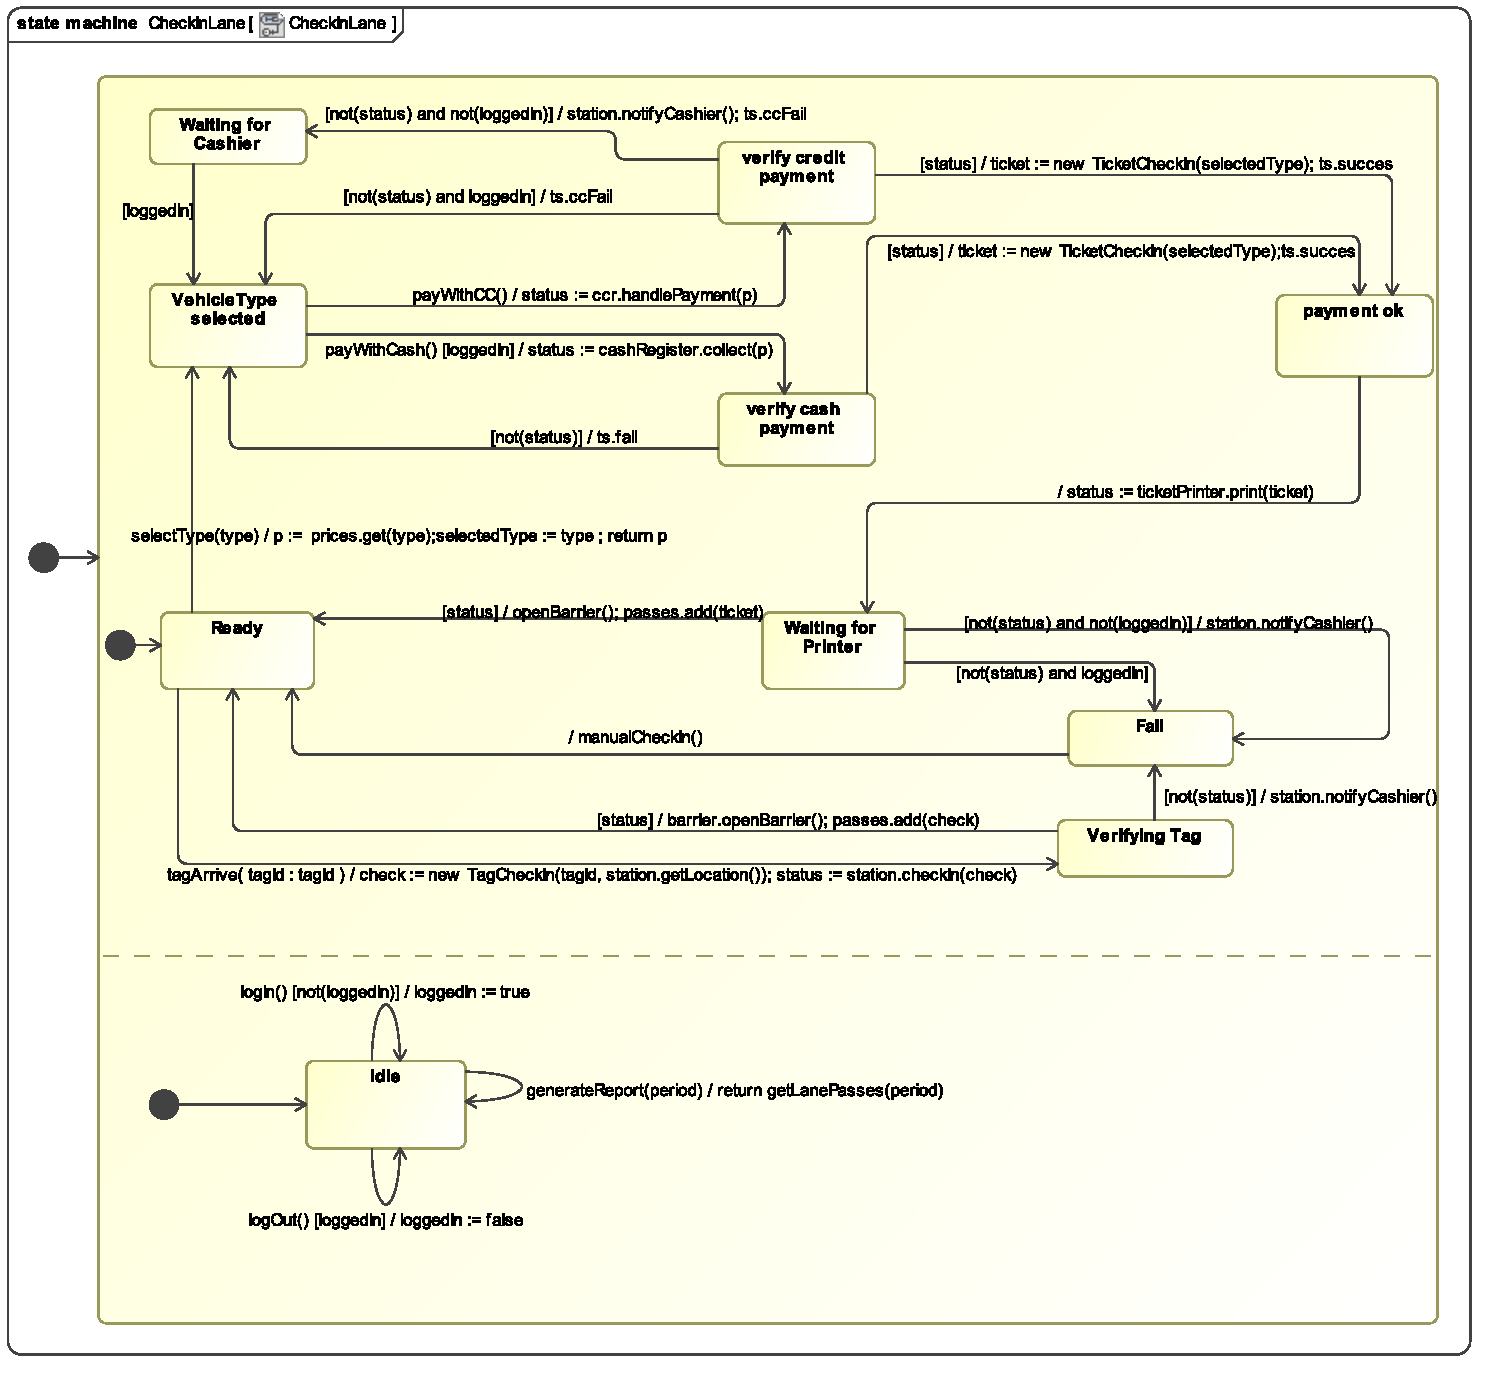
\includegraphics[width=1.0\textwidth,height=0.75\textheight,keepaspectratio, clip=true, trim=0 80mm 0 0]{State_Machine_Diagram/CheckInLane}%
\end{center}
\end{frame}


% % % % % % % % % % % % % % % % % % % % % % % % % % % % % % % % % % % % % % % % % % % % % %

\section{Validation}

\framedgraphic{Sequence: Tag Check-in Success}{Sequence_Diagram/TagCheckIn-Succes}
\framedgraphic{Sequence: Tag Check-in Failure}{Sequence_Diagram/TagCheckIn-Faillure}

\framedgraphic{Sequence: Ticket Check-in Success}{Sequence_Diagram/TicketCheckIn-Succes}
\framedgraphic{Sequence: Ticket Check-in Failure}{Sequence_Diagram/TicketCheckIn-Fail}

\begin{frame}{Design Decisions}
\begin{itemize}
\item Who creates the check-in objects
\item Error handling (true/false vs. enums vs. exceptions)
\end{itemize}
\end{frame}








% % % % % % % % % % % % % % % % % % % % % % % % % % % % % % % % % % % % % % % % % % % % % %
% TEMPLATE STUFF
% % % % % % % % % % % % % % % % % % % % % % % % % % % % % % % % % % % % % % % % % % % % % %
\comm{
\section{Lists}
\begin{frame}
  \frametitle{A slide with a list}
  \framesubtitle{Use <number> to specify layers}
  \begin{itemize}
    \item<1-> First item on all overlays.
    \item<2>  Second item only on the second overlay.
    \item<1,3> Third on first and last.
      \begin{description}
        \item<3>[Note]  Lists can be nested.
        \item<3>[Point] Use this to structure your presentation.
      \end{description}
  \end{itemize}
\end{frame}

\section{Columns}
\begin{frame}
  \frametitle{A slide with columns}
  \begin{columns}[t] % Align the columns at the top
    \column{0.4\textwidth}
      This is the \alert{first} column. It occupies $40$\% of the text width.
    \column{0.6\textwidth}
      This is the \alert{second} column. This could be a nice image\ldots
      \begin{center}
        \rule{0.4\textwidth}{0.3\textwidth}
      \end{center}
  \end{columns}
\end{frame}

\section{Blocks}
\begin{frame}
  \frametitle{Use blocks to highlight your points}
  \begin{block}{<The title of the block>}
    This is the point you want to highlight. It could be an important formula
    \[
      a^2+b^2=c^2
    \]
  \end{block}

  \begin{example}
    The example block is useful for typesetting examples consistently.
  \end{example}
\end{frame}

\section{Verbatim}
\begin{frame}[fragile]
  \frametitle{Verbatim material}
  If the slide contains verbatim material you must use the \texttt{fragile} option for the frame.

  \begin{verbatim}
  This is verbatim text
  !"#�%&/()=?
  \end{verbatim}
  
  The \texttt{listings} package can be used for more fancy verbatim text and pretty printing of source code.
\end{frame}

\section{Finding documentation}
\begin{frame}
  \frametitle{Beamer documentation}
  The Beamer userguide is available on-line at CTAN:
  \begin{center}
    \url{ftp://tug.ctan.org/pub/tex-archive/macros/latex/contrib/beamer/doc/beameruserguide.pdf}
  \end{center}

  If Beamer is installed on your system you can find the manual by running
  \begin{center}
    \texttt{mthelp beamer}
  \end{center}
  in a Command Prompt.
\end{frame}

\section{DTU stuff}

\begin{frame}
  \frametitle{The template}
  This presentation template is a \texttt{beamer} implementation of the official DTU PowerPoint template available at
  \begin{center}
    \url{http://portalen.dtu.dk/Services/Kommunikation.aspx}
  \end{center}
  
  To follow the design guidelines completely, you should use the colors from the DTU color palette
  \begin{center}
    \url{http://portalen.dtu.dk/upload/ak/design/dtu-farvemanual_03_07_2006.pdf}
  \end{center}
  These colors are defined in the DTU beamer theme with the names shown on the next slide.
\end{frame}
  
  \newcommand\dtucolorbox[1]{\parbox[b][1cm+2ex][c]{2cm}{\tiny \centering\color{#1}\rule{.8cm}{.8cm}\\ \textcolor{black}{#1}}}%
\begin{frame}
  \frametitle{DTU colors}
  \centering
  \dtucolorbox{dtudarkgray}\dtucolorbox{dtugray}\dtucolorbox{dtulightgray}\\
  \dtucolorbox{dtudarkblue}\dtucolorbox{dtublue}\dtucolorbox{dtulightblue}\\
  \dtucolorbox{dtured}\dtucolorbox{dtupurpur}\dtucolorbox{dtupurple}\\
  \dtucolorbox{dtudarkorange}\dtucolorbox{dtuorange}\dtucolorbox{dtuyellow}\\
  \dtucolorbox{dtudarkgreen}\dtucolorbox{dtugreen}\rule{2cm}{0pt}\\
\end{frame}

}

\end{document} 
